\section{\texttt{AlphaPhi}: A Generative Model for learning a Tweet's Intrinsic Quality}

For many of us, a tweet is considered a success if we get just a few retweets, since we have just a few followers.
Conversely, some people can get many retweets and consider the tweet a failure, because they have very many of followers and expect more.
We propose the following model that allows us to measure the intrinsic quality of a tweet independent of its visibility.  


\subsection{The model}
We propose the following generative model for retweet behavior on twitter.
Assume that each tweet $s$ has a topic $\tau_s$, known a priori.
We posit that each tweet $s$ has an intrinsic quality $\alpha_s\in [0,1]$, and for each user $u$  and topic $t$ there is a number $\phi_{u,t}$, the probability of user $u$ retweeting a perfect tweet of topic $t$, given that he has seen it.
We then declare
\begin{equation}\label{eq:apeq}
\Prob{\mbox{$u$ retweets $s$}~|~\mbox{$u$ has seen $s$}} = \alpha_s\phi_{u,\tau_s}
\end{equation}
Furthermore we assume every user sees every tweet or retweet posted by one of their friends.

Let $a_{s,u}$ be the binary variable indicating that user $u$ has seen tweet $s$, and $b_{s,u}$ be the binary variable indicating that $u$ has retweeted $s$.
Assume, for now, that $a$ and $b$ can be observed directly from the data.
We can now write down the likelihood function.
\begin{equation} \label{eq:aplikelihood}
l(\alpha,\phi~|~a,b,\tau) = \sum_s\sum_u a_{s,u} \left[b_{s,u}\log\alpha_s\phi_{\tau_s} + (1-b_{s,u})\log(1-\alpha_s\phi_{\tau_s})\right]
\end{equation}


\subsection{Solving the \texttt{AlphaPhi} Problem}

This likelihood (equation~\eqref{eq:aplikelihood}) has a few key properties.  
One is that if $\alpha$ is fixed, the model is additive in the $\phi$, and if $\phi$ is fixed the likelihood is additive in $\alpha$.  
Another is that both conditional subproblems are convex, though the original problem need not be.  
This suggests the following algorithm.  
\begin{algorithm}
  \caption{Estimate \texttt{AlphaPhi} Parameters}
  \label{alg:apalg}

  \begin{algorithmic}
    \State Randomly initialize $\alpha$ and $\phi$.
    \For {$t\in$ Topics}
    \While {Not converged}
    \For {$u\in$ Users}
    \State Optimize $\phi_{u,t}$, holding the rest of the variables fixed.  
    \EndFor
    \For {$s\in$ Tweets with $\tau_s=t$}
    \State Optimize $\alpha_s$, holding the rest of the variables fixed.  
    \EndFor
    \EndWhile
    \EndFor
  \end{algorithmic}
\end{algorithm}
  
To make this practical, we create two files.  
One file lists, for each tweet, how many people retweeted it and the id's of the users that saw but did not retweet.
The other lists, for each user, how many tweets they retweeted and the id's of the tweets they saw but did not retweet.
Each line is enough information to compute the partial derivative of the likelihood with respect to the parameter being optimized.
We compute this derivative at a fixed number of points (say 16) without using any additional memory, and choose the value closest to zero.
Since we can compute the partial derivative of the likelihood in a streaming fashion, this algorithm uses no memory other than what is needed to store current values of the parameters.
The memory requirements are made even easier since we consider only one topic at a time.  
On a Dell laptop with 2GB of RAM, this easily scales to a million tweets and a million users.  

\subsection{Numerical Experiments}

One worries that the likelihood function  (equation~\eqref{eq:aplikelihood}) is not convex!
Indeed, it is easy to find examples where the solution is undefined: for instance if there is a tweet that was never retweeted and only seen by a user that never retweets, clearly the likelihood has no unique maximum.
Still; we plot on, and hope for the best.

Because this is a generative model, it is easy to generate data for experimental purposes, and in fact we might as well assume there is only one topic, since we learn the parameters for each topic separately.  
We start by using the R library \texttt{igraph} to generate a small-world network (Twitter is assumed to be one such).
Then, for each user $u$, we draw $\phi_u$ from a beta distribution.  
We also give each user a randomly selected beta-distribution of their own.  
For each tweet $s$, we randomly pick who the tweeter will be and draw $\alpha_s$ from that user's beta distribution.  
Then, once the parameters are drawn, we simulate the model and output the retweet events.

We ran this simulation on a wide varieties of graph sizes, connectivity levels and parameter generating hyper-parameters, and discovered that, while the problem was technically non-convex, we always found the same optimum regardless of starting point.  
Better yet, the parameters learned were correct: the RMSE over the parameter space was near the theoretical minimum (due to the binning) for even modestly sized problems of several hundred tweets.  

\subsection{Inferring the Twitter Graph}

There is one problem with this model: we need Twitter's follower graph.
Without it, we do not know who has and has not seen a tweet, which is required for the defining equation~\eqref{eq:apeq}.  
Using the retweet graph does not work, as this dramatically overestimates the number of edges in the follower graph.
In particular, a user with relatively few followers who had one tweet go viral will see the rest of his tweets punished, as the actual visibility of the later tweet will be much less than estimated by the retweet graph.  

Thus we wish to estimate the probability that, for users $u$ and $u'$, that $u$ follows $u'$.
The estimate does not have to be perfectly accurate, but cheap and relatively robust.  
Thus, we use a naive bayes assumption, and get
\[\Prob{u\to u'~|~R_{u,u'}\ge r} = \frac{\Prob{u\to u'}\Prob{R_{u,u'}\ge r~|~u\to u'}}{\Prob{R_{u,u'}\ge r}}\]
where $u\to u'$ is a binary random variable indicating $u$ follows $u'$, and $R_{u,u'}$ is the number of times $u$ has retweeted $u'$.  
We know the prior exactly:
\[\Prob{u\to u'}=\frac{F_{u'}}{N}\]
where $N$ is the size of the Twitterati and $F_{u'}$ is the number of followers of user $u'$.
We can estimate $\Prob{R_{u,u'} \ge r}$ directly from the data by building histograms:
\[\Prob{R_{u,u'} \ge r}=\frac{\#\{a : R_{a,u'}\ge r\}}{N-1}\]
The hard part is estimating the likelihood.  For this we make additional, very strong, known-to-be-incorrect assumptions.
We assume that the retweets of a user $u'$ are distributed uniformly among their $F_{u'}$ followers.  
Thus $R_{u,u'}|(u\to u')$ is distributed as binomial with probability $1/F_{u'}$ and $R_u':=\sum_a R_{a,u'}$ trials.  
Even if this assumption were true, it will lead to low-biased estimates of the posterior probability, since some retweets are made by non-followers, and since the assumption is wrong, for the users that don't have most of the retweets, the estimates will be low-biased.
This is actually a good thing: at the very least we won't dramatically overestimate the number of edges while still counting the most adamant followers.  

We get
\begin{eqnarray}
  \Prob{u\to u'~|~R_{u,u'}\ge r} &=& \frac{\Prob{u\to u'}\Prob{R_{u,u'}\ge r~|~u\to u'}}{\Prob{R_{u,u'}\ge r}}\nonumber\\
  &=& \pfrac{F_{u'}}{N}\pfrac{N-1}{\#\{a : R_{a,u'}\ge r\}}\Prob{\mbox{Binomial}(1/F_{u'},R_{u'}) \ge r}\nonumber
abel{eq:edgeprob}
\end{eqnarray}

As a sanity check, if $r=0$, this should be approximately zero.
Indeed it is, as the prior is always approximately zero and normalizer will be approximately 1, thus making the posterior probability extremely small regardless of the likelihood.  
For this reason, if $R_{u,u'}=0$, we set this probability to zero.

Further sanity checking, if $r=1$, for users with few retweets and a reasonable number of followers (average, non celebrity users), this will be high (possibly greater than 1, so we need to clamp!), which is good since we don't expect many retweets from non-followers, so even one retweet means you probably follow that person.  
If $F_{u'}=1$ and only one person retweets, that one person is a follower with probability 1, since the variance in the binomial is zero!  Similar statements remain true if the number of re-tweeters is approximately the number of followers, so for average users this approximation is probably reasonable.  

Now, for any user $u$ and tweet $s$, we have
\begin{eqnarray}
  \Prob{\mbox{$u$ retweets $s$}} &=& \Prob{\mbox{$u$ has seen $s$}}\alpha_s\phi_{u,\tau_s}\nonumber\\
  &=&\left(1-\prod_{u':b_{s,u'}=1}(1-\Prob{u\to u'~|~R_{u,u'}})\right)\alpha_s\phi_{u,\tau_s}\label{eq:apeqfinal}
\end{eqnarray}
where $b_{s,u'}$ indicates $u'$ retweeting $s$, as in equation~\eqref{eq:aplikelihood}.  
We can still optimize individual parameters in Algorithm~\ref{alg:apalg} with only a slight modification; they key properties of the likelihood function still hold.  

\subsection{Features from \texttt{AlphaPhi}: Partial Alphas}

The $\alpha_s$ parameters are, in and of themselves, and interesting feature, since they attempt to tell us how good a tweet is independent of a user's influence.  However, we still with to predict the total number of eventual retweets, so we ask for a little bit more.  
Thus we propose the following predictive features based on this model.     

\label{sec:apfeature}

When a new tweet $s$ is observed at time $p$ after its creation, giving early observations of its retweet behavior, we can (easily) compute estimate $\alpha_s^{(p)}$, which we call the partial $\alpha$ at time $p$. 
We use values of $\alpha_s^{(p)}$ for a few small values of $p$ as high powered features to predict the eventual popularity of $s$.

Another useful feature, given a tweet $s$ of topic $t$ at time $p$ after its creation, is the average value of the $\phi_{u,t}$ for each $u$ that retweeted $s$ so far.
We call this feature $\phi_s^{(p)}$. 

\subsection{Interpreting the parameters}

Not surprisingly, most of the $\phi_{u,t}$'s are zero: most users don't ever retweet things of most topics (some users rarely retweet at all).
In fact, 98.8\% of all the $\phi_{u,t}$ values were zero, while 1.1\% were exactly one.
Explaining the second fact is equally easy: some people retweet almost everything they see from a topic (recall our learning algorithm optimized by binning, so to report a $\phi_{u,t}=1.0$ merely means its closer to 1 than 0.86).  
In the middle, there is a nice spread, as one might expect, see Figure~\ref{fig:phihist}.

Interpreting the $\alpha$ parameters must be done with care, especially when trying to predict the eventual number of retweets.
Indeed, and $\alpha$ can be high both because it was often retweeted and because it was seldom seen.
Users with very few followers often produced these high quality tweets, although many of the most retweeted also had very high quality.
Conversely, a tweet could be low quality because it was over-exposed.  We graph

\begin{figure}[h!]
  \centering
   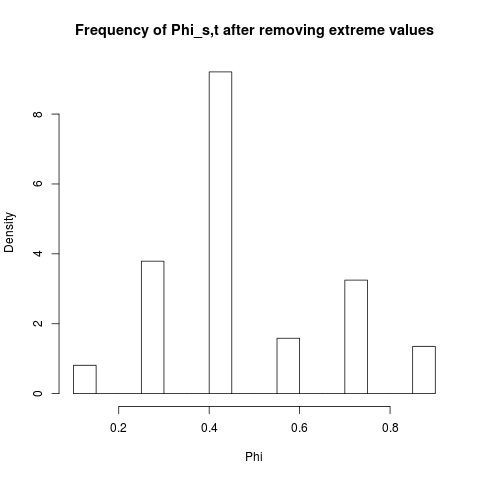
\includegraphics[width=0.5\textwidth]{../src/Analysis/phihist.png}
   \caption{The distribution of the $\phi_{u,t}$ parameters after removing those with values zero or one. }
   \label{fig:phihist}
  
\end{figure}
